% This is samplepaper.tex, a sample chapter demonstrating the
% LLNCS macro package for Springer Computer Science proceedings;
% Version 2.20 of 2017/10/04
%
\documentclass[runningheads]{llncs}
%
\usepackage{graphicx}
\usepackage{todonotes}
\usepackage[hidelinks]{hyperref}
\usepackage{subcaption}
\usepackage{listings}
% Used for displaying a sample figure. If possible, figure files should
% be included in EPS format.
%
% If you use the hyperref package, please uncomment the following line
% to display URLs in blue roman font according to Springer's eBook style:
\renewcommand\UrlFont{\color{blue}\rmfamily}

\begin{document}
%
\title{HERCULES challenge: Identification of topics from Research Objects}
%
%\titlerunning{Abbreviated paper title}
% If the paper title is too long for the running head, you can set
% an abbreviated paper title here
%
\author{Alejandro Gonz\'{a}lez Hevia\orcidID{0000-0003-1394-5073} \and Daniel Fernández Álvarez\orcidID{0000-0002-8666-7660} \and Pablo Menéndez Suárez \and Guillermo Facundo Colunga\orcidID{0000-0003-1283-2763} \and Daniel Gayo-Avello\orcidID{0000-0002-4705-6891} \and Jose Emilio Labra Gayo\orcidID{0000-0001-8907-5348}
}
%
\authorrunning{A. Gonz\'{a}lez Hevia et al.}

\institute{WESO Research Group, University of Oviedo, Spain}

\maketitle

\begin{abstract}
In this paper we propose a system for the extraction of topics from research objects as part of the HERCULES challenge. The system relies on knowledge graphs for the automatic labeling of the topics extracted, and to infer additional topics based on the named entities recognized in each research object. Each topic returned by the system contains semantic information with references to other vocabularies and its assigned confidence score. For the evaluation of the topics we rely on standard measures such as perplexity and topic coherence, but also propose new metrics based on the semantic similarity between the topics predicted by the system and a baseline. Methods for the automatic summarization of research objects are also proposed. All of the results can be provided by the system following Semantic Web formats, and additional steps for the improvement in the system in future versions are also addressed. Source code repositories and models created in this challenge are also provided as part of this paper.

\keywords{natural language processing \and topic modeling \and linked data \and knowledge graph \and text summarization}
\end{abstract}
%
%
%
\section{Introduction}
The HERCULES project\footnote{\url{https://www.um.es/web/hercules/}} has been proposed as a University Research Data Semantics system for Spanish universities with the goal of developing new semantic  web technologies that gather new  information and integrate multiple nodes with heterogeneous ontologies and vocabularies. The University of Murcia (hereinafter UM) signed an agreement with the Spanish Ministry of Economy, Industry and Competitiveness (MINECO) in 2017 backing the HERCULES project with an 80\% of cofinancing from the European Regional Development Fund program (ERDF) within the 2014-2020 period. The purpose of this agreement was to establish collaboration amongst MINECO and the UM,  directed towards the improvement of public services and business innovation through the Public Procurement of Innovation. Some goals of the system were to create a research management system with semantic capabilities and infrastructures and create support systems for the detection of synergies in R\&D between universities. The HERCULES project was divided in three main sub-projects: semantic architecture and ontological  infrastructure, research management system; and data enrichment and methods of analysis.

In this paper we present the system developed as part of the Herculles challenge of EDMA, which belongs to the data enrichment and methods of analysis sub-project. The main objective of the Hercules Challenge is the extraction of topics that describe a Research Object (RO), and the use of those topics to generate a researcher profile based on their RO production. The challenge is divided into 3 main tracks related to three different kinds of research objects: Publications, Experimental Protocols and Git Repositories. Results obtained for each track must be expressed using a common model based on Linked Open Data.

This paper is structured as follows: In section~\ref{related_work} we will go over the related work in the field of topic extraction and automatic topic labeling. Section~\ref{datasets} will describe the datasets that form part of the challenge. In section~\ref{proposed_approach} we will give an overview of the system proposed for this challenge, and explain the functionality of its components. The techniques used for the evaluation of each track and the final hyperparameters chosen are detailed in section~\ref{evaluation}. In section~\ref{future_work}, we will go over some of the functionality that could be further analysed and implemented in future versions of the system. Finally, we will give our final conclusions and links to the source code repositories in section~\ref{conclusions}. 

\section{Related Work} \label{related_work}
There has been an interest for the past years in developing efficient text mining and recommendation systems for scientific articles. Latent Dirichlet Allocation topic models are the most used in this area of study \cite{tong2016text,younus2014utilizing,jelodar2019natural,jelodar2019latent}. However, the main problem of these types of topic models is that a distribution of terms is returned for each topic and normally a manual annotation of the topics with a label which can be better understood by humans is required.

Several approaches to perform automatic topic labeling have been proposed to solve this problem. Mei et al. \cite{mei2007automatic} formulate the problem of topic labeling and the main phases it is composed of: candidate label generation and candidate label ranking. Lau et al. \cite{lau2010best} propose the use of one of the top 10 words to represent each topic. Six different features are fed to a support vector regression model to rank the best word to be used as a topic label. Hulpus et al. \cite{hulpus2013unsupervised} makes use of DBPedia to generate the candidate labels, and proposes a set of centrality measures to rank the candidates. The use of neural embeddings, like word2vec, obtained from Wikipedia articles has also been studied to extract candidate labels for each topic \cite{bhatia2016automatic}.

Regarding the automatic extraction of topics from source code, Chen et al. \cite{chen2016survey} surveyed several articles regarding the use of topic models for software engineering tasks. They found out that most studies focus on only a limited number of software engineering tasks and only basic topic models are used in those tasks. Some variants of LDA, such as Latent Semantic Analysis (LSA) \cite{deerwester1990indexing}, Independent Component Analysis (ICA) \cite{hyvarinen2000independent} and Probabilistic Latent Semantic Analysis (PLSA) \cite{hofmann2013probabilistic} are also proposed.

With respect to the representation of this topics following Semantic Web principles, several vocabularies and representation formats have been proposed. One of those is the Lexicon Model for Ontologies (LEMON) \cite{cimiano2016lexicon}, which was proposed as a way of modeling lexicon and machine-readable dictionaries. Hellman et al. \cite{hellmann2013integrating} proposed the NLP Interchange Format (NIF) to achieve interoperability between Natural Language Processing tools, language resources and annotations. Finally, Cimiano et al. \cite{cimiano2015linked} propose another approach for publishing and linking terminological resources combining the LEMON, SKOS and PROV-O vocabularies in their core model.

\section{Datasets} \label{datasets}
The following datasets have been used as part of this challenge:
\begin{itemize}
	\item Publications: For this track, the dataset consists of 125 agriculture publications from EuropePMC\footnote{\url{https://europepmc.org}}. The dataset was fetched using the Europe PMC API\footnote{\url{https://europepmc.org/RestfulWebService}}, and each publication contains its title, content and list of authors.
	\item Protocols: In this case, the dataset consists of 100 open-access experimental protocols from Bio-Protocol\footnote{\url{https://bio-protocol.org/Default.aspx}}. Each protocol is composed of an abstract, list of materials, list of equipment, its procedure and the list of authors.
	\item Git: This dataset consists of 50 GitHub repositories. The contents were fetched using the GitHub API\footnote{\url{https://docs.github.com/en/rest}}. For each repository the title, description, issues, commits, languages and source code was fetched. In  \figurename~\ref{git_languages} we can see the top 10 programming languages from this dataset. Overall, there is not a main programming language shared amongst every repository, and many different technologies are being used. It is important to note that only two of the repositories contain issues, and 3 of them don't have neither a readme nor a description, so the amount of information available in natural language is scarce. In some cases, it may be needed to perform some kind of code analysis in order to enrich the information extracted from the research object. 
\end{itemize}

\begin{figure}[h]
	\begin{center}
	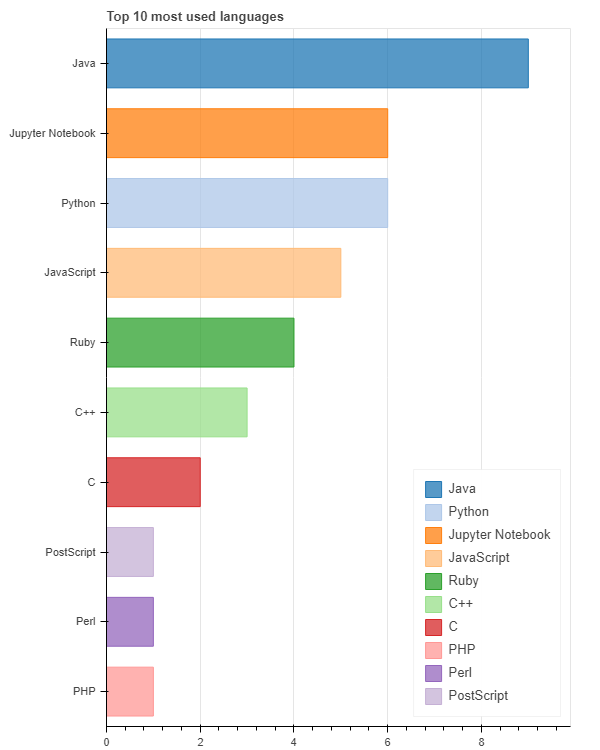
\includegraphics[width=0.65\textwidth]{img/git_languages.png}
	\caption{Top 10 programming languages from the Git dataset.} \label{git_languages}
	\end{center}
\end{figure}


\section{Proposed approach} \label{proposed_approach}
\subsection{System overview}
In \figurename~\ref{complete_system} the general pipeline of operations that will be executed on a research object to obtain its associated topics is illustrated. We can distinguish between two main pipelines that can be executed in parallel: the first one will obtain a list of topics based on the named entities identified in the text, and the second one will make use of topic models to obtain the list of topics. After these lists of potential topics are identified, they will be combined and returned by the sistem. For now, we will go over the main steps that compose each pipeline. Singularities related to every track will be described in the following sections.

\begin{figure}[h]
	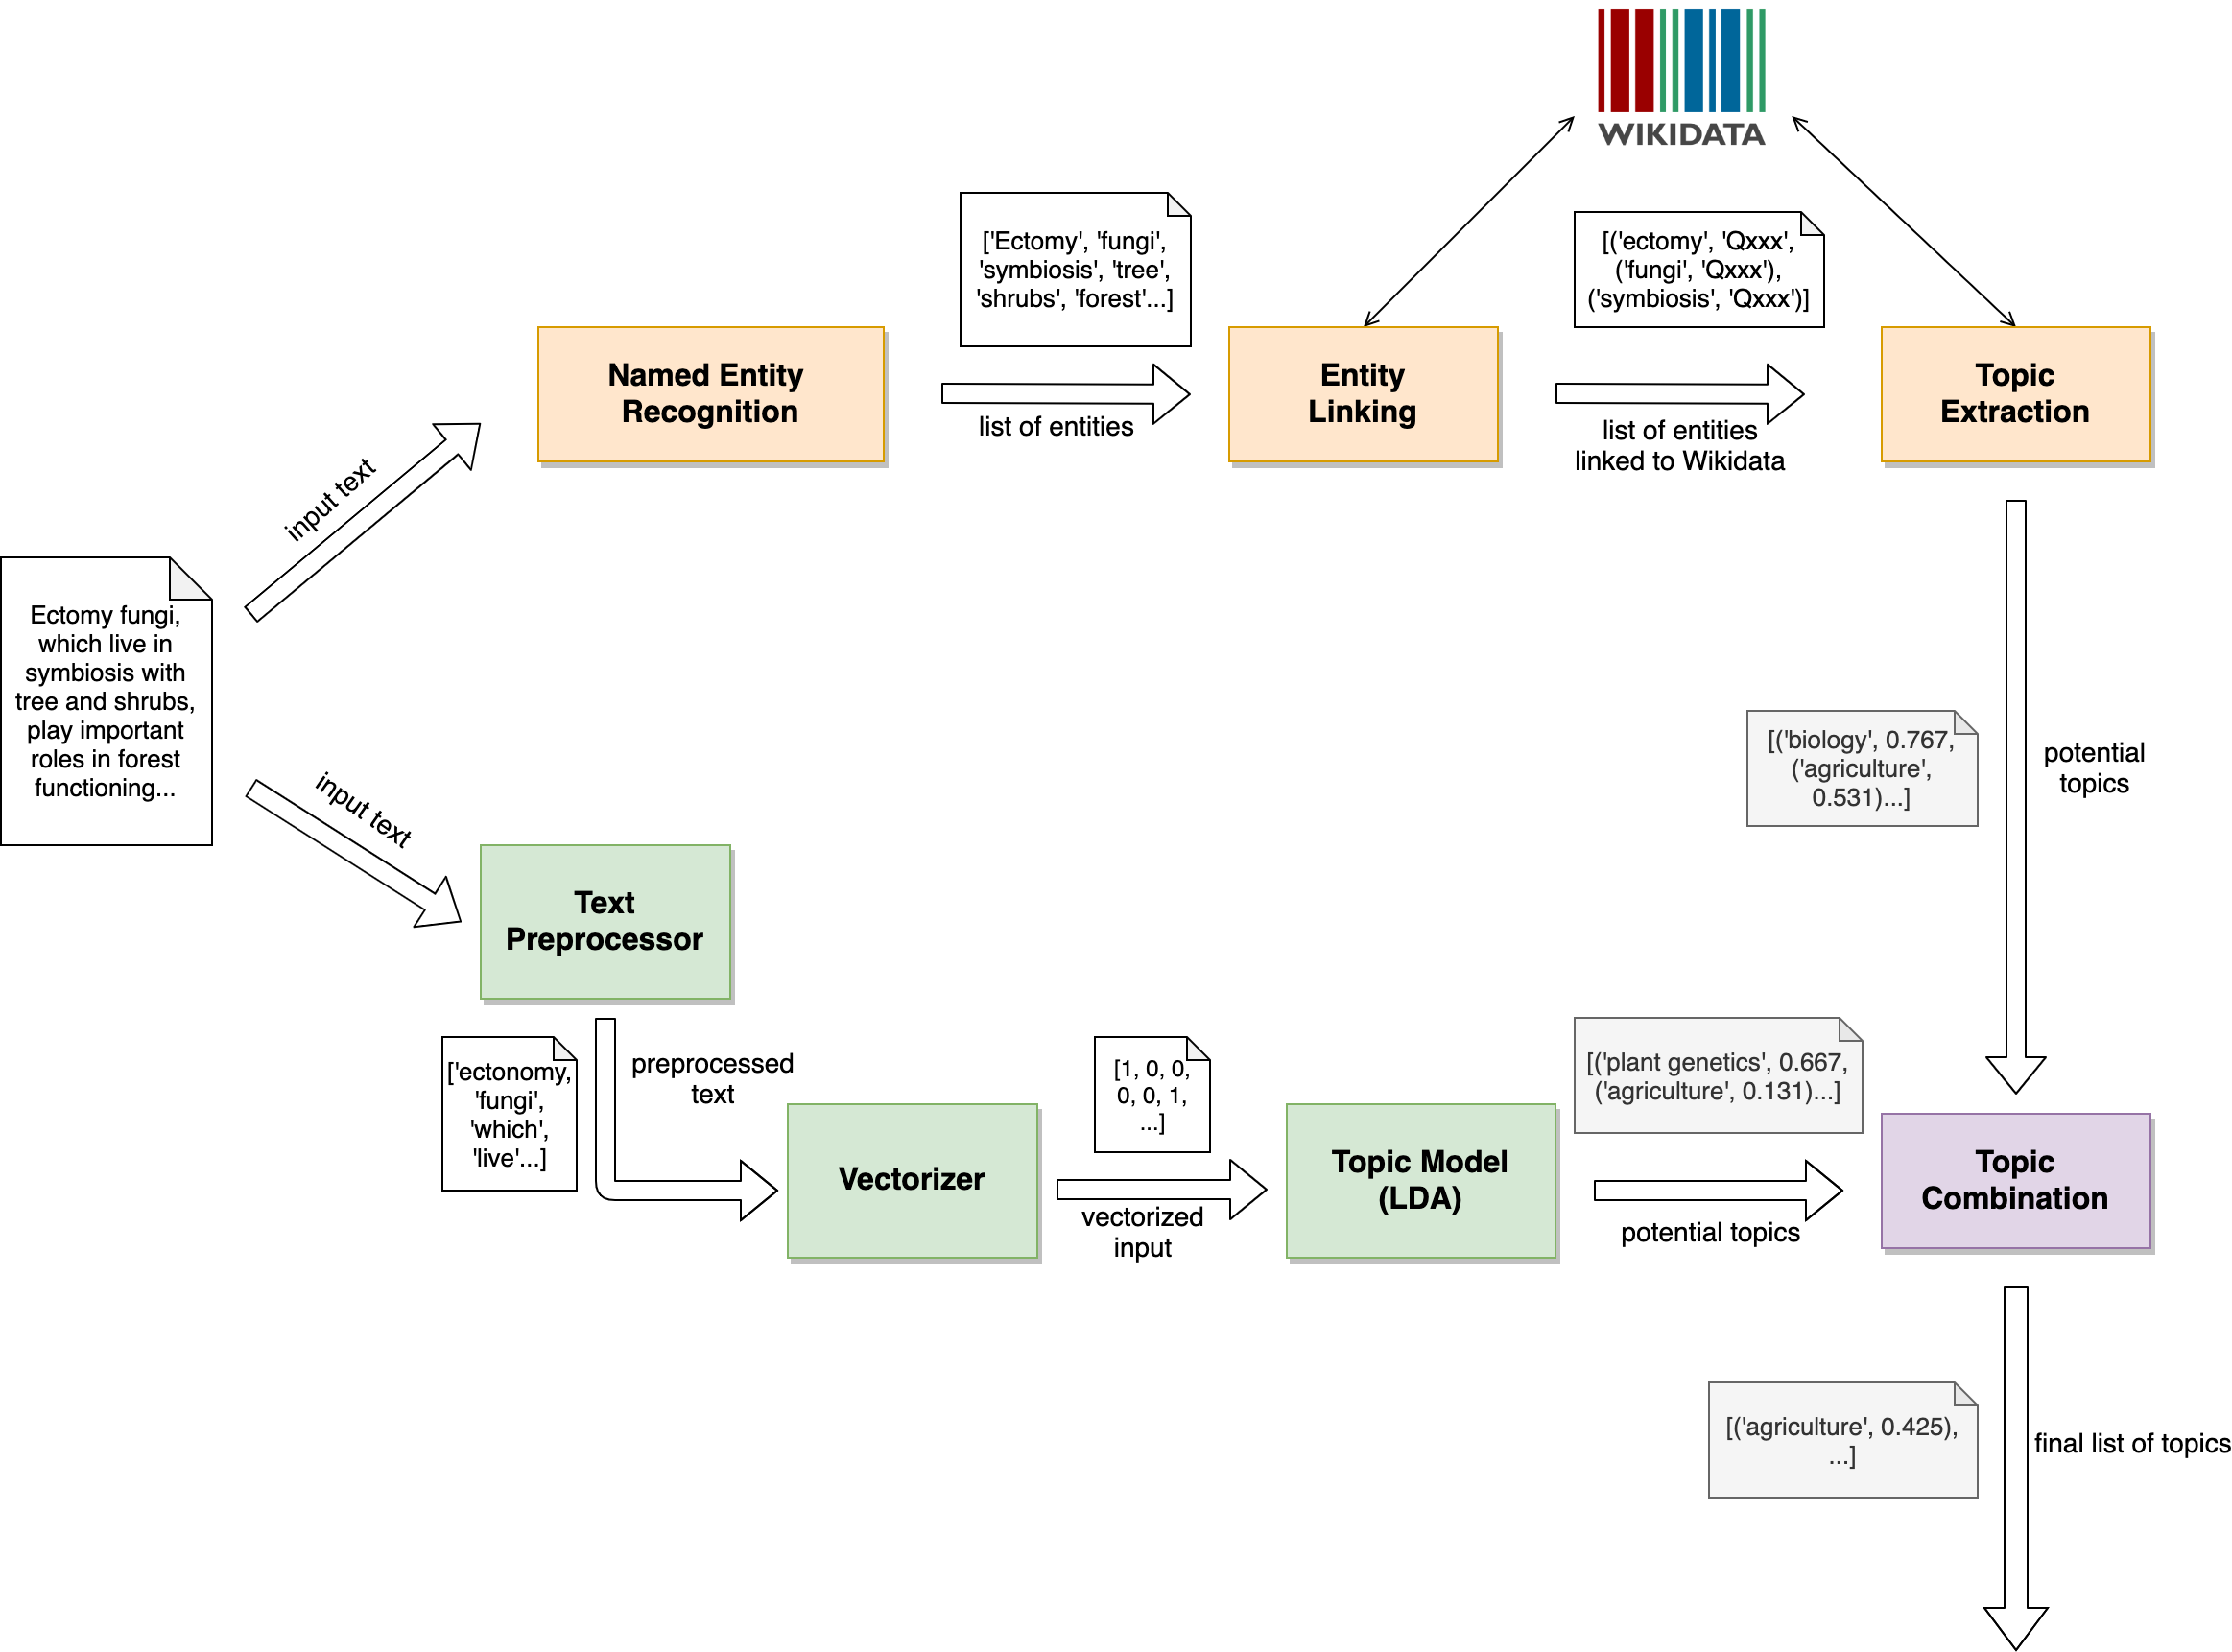
\includegraphics[width=\textwidth]{img/complete_system.png}
	\caption{General flow of data for the topic extraction system.} \label{complete_system}
\end{figure}

\subsubsection{Topic extraction from topic models.}
This pipeline will make use of different topic modeling algorithms to obtain a list of topics from the research objects. It is composed of the following steps:

\begin{itemize}
	\item \textbf{Text Preprocessing}: In this step the input text is normalized and tokenized before reaching the following filters. Spacy\footnote{\url{https://spacy.io}} is used for the tokenization, lemmatization and expansion of abbreviations from the input text. We have explored both the default Spacy models and the scispaCy\footnote{\url{https://allenai.github.io/scispacy/}} models trained with scientific and clinical texts \cite{neumann-etal-2019-scispacy}. A default stop word list is also used, but it is also customized and expanded with domain-specific stop words for every track. 
	\item \textbf{Vectorization}: This step encompasses the conversion of the processed tokens into a numerical representation that can be consumed by the machine learning models from the following steps. Depending on the track and machine learning model to be used, different vetorized outputs can be produced\footnote{Some examples of vectorized outputs from this step can be TF, TF-IDF or Word2Vec embeddings.}.
	\item \textbf{Topic model}: Once a vectorized input has been computed, it will be fed into a topic modeling algorithm to infer the topics of the text with their associated probabilities. In this challenge we have explored the use of Latent Dirichlet Allocation (LDA) \cite{blei2003latent}, Non-Negative Matrix Factorization (NNMF) \cite{xu2003document}, Latent Semantic Analysis (LSA) \cite{deerwester1990indexing} and CorEx \cite{gallagher2017anchored}. Results obtained with each model and the optimum set of hyperparameters will be defined in the following sections. It is important to note that other topic modeling techniques can be easily explored and integrated into the pipeline. 
	
	Every topic model named aboved returns a list of topic described by their term distribution. However, none of the topics contain a label that could be interpreted by humans. This step, known as topic labelling, is usually done manually or semi-manually by a set of domain experts. In our approach, we propose an automatic labelling technique based on the exploration of knowledge graphs. To obtain a label for each topic, we rely on its top n words based on their relevance \cite{sievert2014ldavis}, which from now on will be called \textit{seed terms}. The $n$ and $\lambda$ parameters used in this step are optimized for each track. This set of seed terms are linked to Wikidata, and a graph of terms is created by exploring their neighbourhood terms with the use of a set of Wikidata properties to be expanded\footnote{For example, this set contains the \textit{instance of} property (P31), and therefore every \textit{instance of} predicate from the set of seed terms would be expanded to build their neighbourhood graph.}. After this step we may either obtain a list of subconnected graphs of a unique graph with every seed term. If there are more than one subgraphs, we select the largest connected subgraph to be used for the following steps. Usually, small subgraphs formed by a single or small number of seed nodes may indicate a set of terms that are not completely related to the topic and should be ignored.
	
	Once the final subgraph is obtained, we apply a series of centrality algorithms on the graph in order to identify the most "relevant" entities that best describe the topic graph that has been built. The entity that receives the best centrality score is then used as a label for the given topic. These stepsare repeated for all the topic distributions inferred by the topic model to obtain their labels. 
	
	Then, whenever we obtain the probability distribution for every topic with a new document, we will already have an associated label for the topic. The output of this step will be a list of labelled potential topics of the given research object with their associated probabilities.
\end{itemize}

\subsubsection{Topic extraction from named entities.}
In this pipeline, the list of potential topics will be obtained based on the named entities recognized in the research object. It is composed of the following phases:

\begin{itemize}
	\item \textbf{Named Entity Recognition}: This step will receive an input text from a research object and apply Named Entity Recognition techniques to extract its entities. General named entity recognition models from spaCy and scientific ones from scispaCy are used. Since the main entities that compose the topics of the research object will tend to be repeated more than once along the whole object, a parameter was configured to remove entities with less appearances than its value. The output of this phase will be the list of entities identified in the research object.
	\item \textbf{Entity linking}: In this step we disambiguate the entities extracted before by linking them to a knowledge base. Depending on the ontology that we will be linking the entities against, this process might change. For the purposes of this challenge, we are using both DBPedia and Wikidata as the default knowledge bases where the entities are linked against, and topics are extracted from. The main difference between this entity linking step and the one performed previously in the topic labelling step is that in this case we have available the complete text where the entities are located to perform a better disambiguation, while in the previous case we could only rely on the isolated terms that compose a topic.
	
	For this initial implementation of the system we are using the DBPedia Spotlight \cite{mendes2011dbpedia} service to link the entities against DBPedia, and the Wikidata API to link them against Wikidata. Other domain-specific ontologies to be used in this phase and the following one can be integrated in this architecture. The output of this phase will be a list of disambiguated entities with their associated Wikidata URI\footnote{For entities disambiguated using the DBPedia Spotlight service, we explore their associated owl:sameAs predicate to find their Wikidata URI.}.
	\item \textbf{Topic extraction from the linked entities}: Once we have a list of entities linked against Wikidata, our next step is the exploration of the graph formed by those entities and their neighbourhood to obtain a list of entities that represent potential topics of the research object. The same algorithm and substeps are used for the graph building and exploration as the ones described in the automatic topic labeling step. The output of this step will be the potential list of topics inferred for the research objects with their associated confidence score. These topics are annotated with semantic information retrieved from their Wikidata entity.
\end{itemize}

\subsubsection{Topic combination.}
After the two lists of potential topics from the pipelines has been produced, the final step consists of merging them and returning the final list of topics. In this step of topic combination, a weight is applied to each pipeline to give a higher priority to results obtained from one pipeline or another. A score threshold can also be configured to return only those topics that have a confidence score above that threshold.

Once the final list of topics is obtained, we make use of the NIF vocabulary\footnote{\url{https://persistence.uni-leipzig.org/nlp2rdf/}} and the semantic information for each entity from Wikidata to provide an output in multiple Semantic Web formats\footnote{Currently the turtle, RDF/XML, n3 and JSON-LD formats are supported.}. A minimal example of the results returned by the system for a given GitHub repository can be seen in \figurename~\ref{output_example}. The string used by the system to infer the topics, its predominant language and source url are included. For each topic that has been inferred, we provide its labels and descriptions in multiple languages, a link to the topic entity in other ontologies and thesauri, and the confidence value returned by the system.

\begin{center}
\begin{lstlisting}[tabsize=2, breaklines=True, basicstyle=\footnotesize\ttfamily,]
edma:103798851 nif:isString "Algorithms in C Language..." ;
	nif:predominantLanguage "en" ;
	nif:sourceURL <https://www.github.com/...> ;
	nif:topic [ a nif:annotation ;
		rdfs:label "algorithm"@en,
					     "algoritmo"@es ;
		rdfs:comment "unambiguous specification of how to..."@en,
							   "procedimiento e instrucciones para..."@es ;
		itsrdf:taIdentRef <http://id.nlm.nih.gov/mesh/G17.035>,
			<https://academic.microsoft.com/v2/detail11413529>,
			<https://freebase.toolforge.org//m/0jpv>,
			<https://meshb.nlm.nih.gov/record/ui?ui=D000465>,
			<https://www.wikidata.org/w/Q8366> ;
		nif:confidence 9.596685e-01 ] .
\end{lstlisting}

\captionof{figure}{Example output of the system for a given repository.}
\label{output_example}
\end{center}


\subsection{Publications track}
For the publications track, we used as input features for our model the title, abstract and content of each publication. A custom domain-specific stopword list was created to complement the default one from spaCy. An additional phase was added to the complete system, which performed a grouping of the topics per author and returned the most relevant topics considered for each author. 

\subsection{Protocols track}
Regarding the protocols track, the input fed to our models was the title, abstract, list of materials and equipment, and procedure of the protocol. An additional requirement for this track was to implement an automatic summarization technique for protocols. The abstract of each protocol was used as a baseline to compare our results against. The following two types of summaries were created:
\begin{itemize}
	\item Extractive summaries: This type of summarization consists on identifying important sections of the text to be summarized, and using those sections to generate the final summary. In this case no new text is generated by the technique, and the summary will always be a subset of the sentences from the original text.
	
	For this approach, we implemented a TF based technique to obtain the most relevant sentences of the protocol. The sentences were identified and tokenized using SpaCy, and we calculated the term frequency of each term in the text and aggregated those values to obtain a final relevancy score of each sentence. The top $n$ most relevant sentences were then combined to produce the final summary of the protocol.
	
	\item Abstractive summaries: This type of summarization can reuse some of the sentences from the original text, but can also generate new text to produce the final summary of the input text. Our approach for this type of summarization was to make use of pretrained BART \cite{lewis2019bart} models and finetune them for this specific track. In our experiments we trained following models:
		\begin{itemize}
			\item \texttt{bart\_cnn}: Bart model trained on the CNN/Dailymail summarization dataset\footnote{\url{https://www.tensorflow.org/datasets/catalog/cnn_dailymail}}. This is a general purpose model used as a baseline to be compared againts the finetuned approaches.
			\item \texttt{distilbart\_cnn}: This is a model where alternating layers of the bart-large-cnn model are copied and the others are finetuned on a subset of protocols. The abstract of each protocol was used as the target text to be inferred from the rest of information.
			\item \texttt{distilbart\_xsum}: This model follows the same principles as the previous one, but the base model was trained on the extreme summarization (XSum)\footnote{\url{https://www.tensorflow.org/datasets/catalog/xsum}} dataset instead of the CNN one.
		\end{itemize}
\end{itemize}

\subsection{Git track}
Regarding the git track, as explained in the datasets section one of the main difficulties was to obtain a complete set of input features to be used by the topic extraction system. The use of information from source code was a necessity due to the lack of readme and description in some repositories. We performed several experiments with the use of comments from the source code (both inline and multiline) as additional input for the system, but the overall performance of the system worsened as a result. The use of source code identifiers both at a class and function level has also been used in previous approaches of topic extraction from source code. However, due to the variety of programming languages the development of language-specific parsing tools was not possible for this challenge, but remains as future work. Our final list of input features was composed of the description of each repository, contents of the readme (if available), commits, and the list of names of each source code file\footnote{Multiword file names written in \texttt{CamelCase} and \texttt{snake\_case} were separated into their single words.}.

This dataset also posed an additional challenge when disambiguating entities with respect to the other tracks\footnote{Many software engineering tools tend to have ambiguous names. E.g. \texttt{Cucumber}, \texttt{pandas}, \texttt{gatling}...}. Due to this, we obtained better results when using the DBPedia Spotlight service to disambiguate the entities from the repository.

\section{Evaluation of results} \label{evaluation}
In this section we will go over the evaluation method and results of the proposed system for this challenge. We will start by explaining the general method of evaluation shared amongst all of the tracks, and then we will go over the evaluation of each track.

\subsection{General method}
For the evaluation and hyperparameter tuning of the topic extraction models we used perplexity and topic coherence measures amongst all tracks. \figurename~\ref{coherence_tracks} illustrates the evolution of topic coherence with different number of topics for the best topic models of each track.

\begin{figure}
	\centering
	\begin{subfigure}[b]{0.45\textwidth}
		\centering
		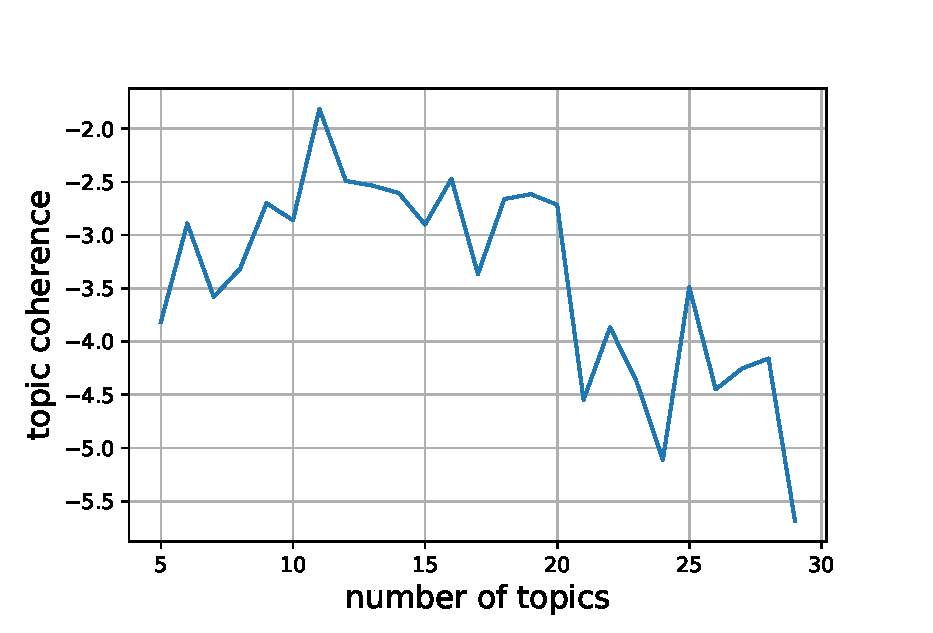
\includegraphics[width=\textwidth]{img/protocols_coherence.eps}
		\caption{Protocols track (LDA unigrams)}
	\end{subfigure}
	\hfill
	\begin{subfigure}[b]{0.45\textwidth}
		\centering
		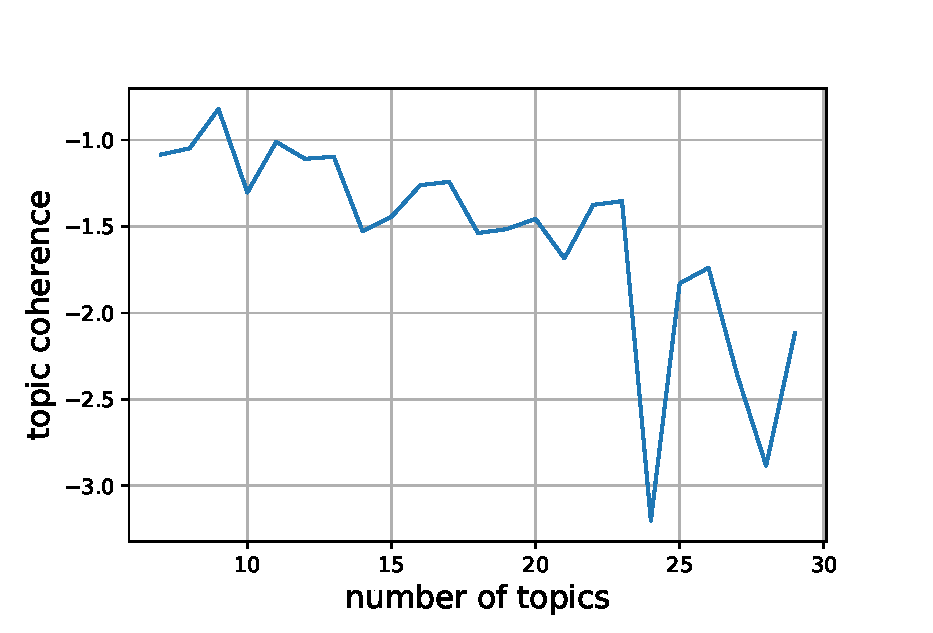
\includegraphics[width=\textwidth]{img/publications_coherence.eps}
		\caption{Publications track (LDA unigrams)}
	\end{subfigure}
	\hfill
	\begin{subfigure}[b]{0.45\textwidth}
		\centering
		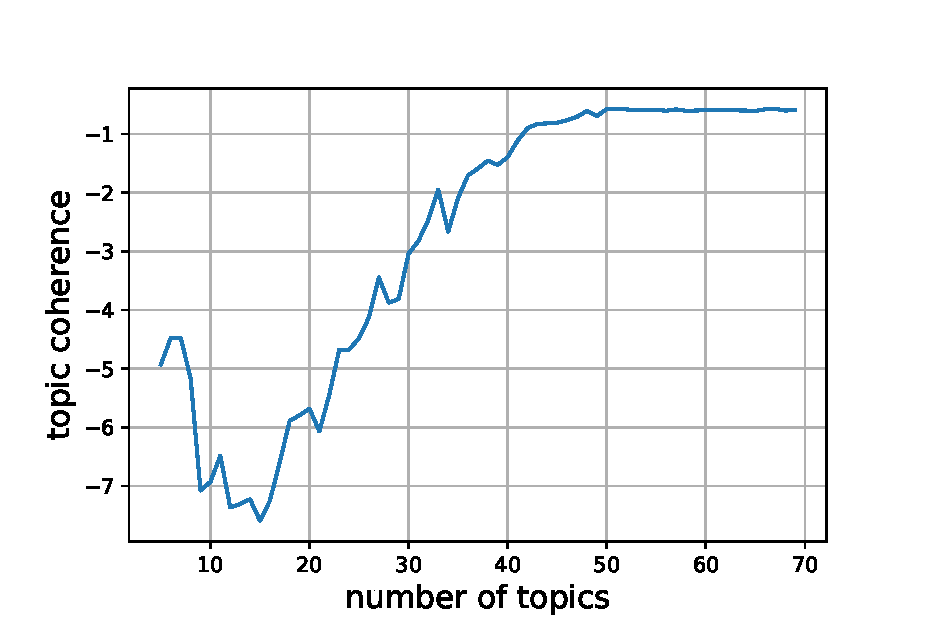
\includegraphics[width=\textwidth]{img/git_coherence.eps}
		\caption{Git track (NMF bigrams)}
	\end{subfigure}
	\caption{Topic coherence evolution with number of topics}
	\label{coherence_tracks}
\end{figure}

For the evaluation of the final system, we relied on measuring the semantic similarity between the topics predicted by the system and a set of topics for each track regarded as ground truth. For each instance of the dataset, we calculate the semantic similarity between each topic returned by the system and the base topics. This similarity is calculated using the Leacock-Chodorow similarity metric \cite{budanitsky2001semantic} using the WordNet interface provided by NLTK\footnote{\url{https://www.nltk.org/howto/wordnet.html}}. With every similarity value obtained we build an $n \times m$ matrix with each row being a topic predicted by the system and each column a ground truth topic. Each value $x_{nm}$ in the matrix equals to the semantic similarity score calculated between topics $n$ and $m$. This matrix is then used to perform an association between every predicted topic to a ground truth one. Once these associations have been made, we compute the min, max, median and mean semantic similarity of the associations. This step is repeated for every instance in the dataset to compute the final similarity scores of the system in each track.

\subsection{Publications track}
For the publications track, we used as ground truth topics the categories returned by the EuropePMC API. Some of the categories were too general\footnote{For example, 'Research Article', 'Original Paper' and 'Article'.}, so we performed an additional step of manual cleaning before using them as ground truth labels. After the cleaning step, only 26 publications from the original set of 126 had one or more categories to be used as ground truth. This sample was used to optimize the hyperparameters of the system. The best results were obtained with unigrams, a LDA model with 9 components, and a 0.8 relevance score to get the top n words of each topic.

\subsection{Protocols track}
For the protocols track, we used the subjects of each protocol as ground truth topics to compare our results against. In this case, after a manual inspection of the subjects no removal of topics was needed. From the original dataset of 100 protocols, 96 of them had one or more ground truth topics.  The best results for this dataset were obtained with unigrams, a LDA model with 11 components, and a 0.8 relevance score.

\subsection{Git track}
For the git track, since none of the GitHub repositories had topics associated to it we had to perform a manual annotation of topics. Three people annotated the dataset with those topics that they considered relevant based on a set of general guidelines, and then the three annotated datasets were merged into a final dataset. For the merging process we selected as ground truth labels for each repository those topics which were chosen by at least two of the annotators. The best results for this dataset were obtained with bigrams, a NMF model with 50 components, and a 0.9 relevance score.


\section{Future Work} \label{future_work}
\subsection{Improvement of entity linking techniques}
For the purposes of this challenge we relied on the DBPedia Spotlight service and the Wikidata API to link entities to DBPedia and Wikidata respectively. However, several improvements can be made to these approaches. For example, the use of collective disambiguation, where the type of the most confident entities that have been linked can be used to disambiguate future entities from the text, has been shown to improve results from DBPedia Spotlight\cite{chabchoub2018ficlone} and can be implemented in future versions of the system.

Regarding the linking of entities to Wikidata, SpaCy has recently added support for the creation of Knowledge Bases\footnote{\url{https://spacy.io/api/kb}} and training of custom entity linking models. They are currently working on native support for Wikidata, and there is already the possibility of training a custom entity linking model using texts from Wikipedia\footnote{For more information, see \url{https://bit.ly/324uDKP}}. The exploration of these techniques is left as future work for the following versions of the system.

\subsection{Performance improvements}
With the current system implementation, there is a bottleneck in the creation of the neighbourhood graph from the set of seed terms that is used in the topic extraction from named entities. This is due to the number of external calls that need to be done to Wikidata to fetch the complete set of nodes that compose the final graph. The performance of the system could greatly increase if we index the ontology in a system like ElasticSearch\footnote{\url{https://www.elastic.co/elasticsearch/}}. We could deploy the system in a custom machine and perform our queries against it. Since the entire dump of Wikidata is also really big (the JSON dump has more than 1TB of size), and most of the information may not be used for the extraction of topics from research objects\footnote{An example of the item distribution in Wikidata is available at \url{https://www.wikidata.org/wiki/Wikidata:Statistics}}, there is also the possibility of creating subsets of Wikidata with those entities that will be desired to have available.

\subsection{Implementation of additional graph centrality algorithms}
In order to obtain a list of potential topics from the graph that has been built, several graph centrality algorithms were used\footnote{Information centrality, Closeness centrality, eigenvector centrality and betweenness.}. However, Hulpus et al \cite{hulpus2013unsupervised} propose a new set of centrality measures to obtain the most relevant entities based on the ones that have been used. The implementation and evaluation of these new algorithms is a functionality that can be addressed in future versions of the system.


\section{Conclusions} \label{conclusions}
As part of this paper we have presented our system for the extraction of topics for the HERCULES challenge. We relied on the use of knowledge graphs as a tool to perform an automatic labeling of the topics infered by the systems, and as a way to obtain aditional topics from the named entities recognized in each Research Object. The use of a knowledge graph allows us to obtain semantic information about the extracted topics which can then be reused to return the system results following Semantic Web formats.

For the evaluation of our system we relied on the perplexity and topic coherence scores of the topic distribution inferred by each model, but also generated semantic similarity scores between the topics inferred by our system and a baseline for each track.

The development of common code for the challenge has been made on the \textit{hercules\_challenge\_common}\footnote{\url{https://github.com/weso-edma/hercules-challenge-common}} GitHub repository. The development of the Publications, Protocols and Git tracks was made on the \textit{hercules\_challenge\_publications}\footnote{\url{https://github.com/weso-edma/hercules-challenge-publications}}, \textit{hercules\_challenge\_protocols}\footnote{\url{https://github.com/weso-edma/hercules-challenge-protocols}} and \textit{hercules\_challenge\_git}\footnote{\url{https://github.com/weso-edma/hercules-challenge-git}} repositories respectively. Source code, models, and instructions to run each system and reproduce our results can be found in those repositories.

\bibliographystyle{splncs04}
\bibliography{bibliography}
\end{document}
